\documentclass{standalone}
\usepackage{tikz}

\begin{document}
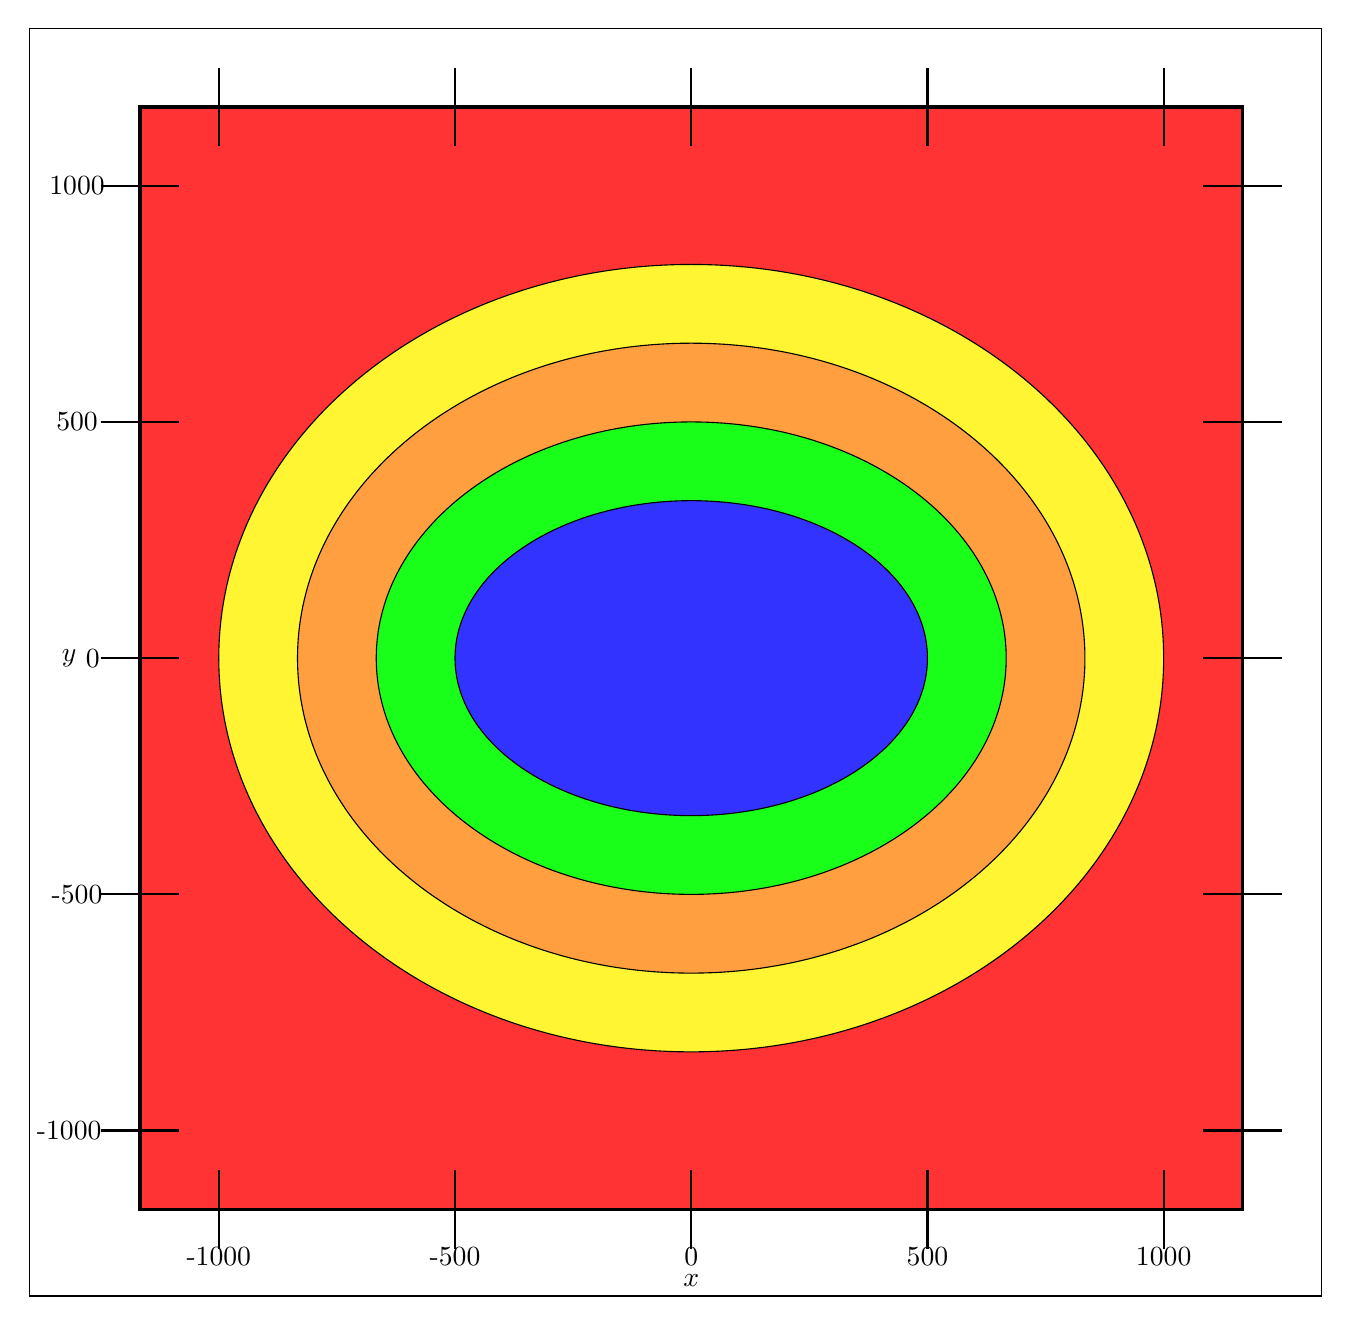
\begin{tikzpicture}

%draws background and ellispes
\draw[fill=white] (-8.4,-8.1) rectangle (8,8);
\draw[fill=red!80,very thick] (-7,-7) rectangle (7,7);
\draw[fill=yellow!80] (0,0) ellipse (6 and 5);
\draw[fill=orange!75] (0,0) ellipse (5 and 4);
\draw[fill=green!90] (0,0) ellipse (4 and 3);
\draw[fill=blue!80] (0,0) ellipse (3 and 2);

%draw grid
\foreach \x in {-6,-3,...,6}
    \draw[thick] (\x,-7.5) -- (\x,-6.5)  (\x,7.5) -- (\x,6.5);
\foreach \y in {-6,-3,...,6}
    \draw[thick] (-7.5,\y) -- (-6.5,\y) (7.5,\y) -- (6.5,\y);

%label grid
\draw (-6,-7.6) node {-1000};
\draw (-3,-7.6) node {-500};
\draw (0,-7.6) node {0};
\draw (0,-7.9) node {$x$};
\draw (3,-7.6) node {500};
\draw (6,-7.6) node {1000};

\draw (-7.9,-6) node {-1000};
\draw (-7.8,-3) node {-500};
\draw (-7.6,0) node {0};
\draw (-7.9,0) node {$y$};
\draw (-7.8, 3) node {500};
\draw (-7.8, 6) node {1000};
\end{tikzpicture}
\end{document}